\documentclass[border={20.000000bp 20.000000bp 20.000000bp 30.000000bp}, 11pt]{standalone}
\pdfinfoomitdate=1
\pdftrailerid{}
\pdfsuppressptexinfo=1
\pdfinfo{ /Creator () /Producer () }

\usepackage{tikz}
\usepackage{xcolor}
\usetikzlibrary{shapes.misc}
\usetikzlibrary{backgrounds}

\definecolor{dotColorA}{HTML}{1F77B4}
\definecolor{dotColorB}{HTML}{1F77B4}
\definecolor{dotColorC}{HTML}{1F77B4}
\definecolor{dotColorD}{HTML}{1F77B4}
\definecolor{dotColorE}{HTML}{1F77B4}
\definecolor{dotColorF}{HTML}{1F77B4}
\definecolor{dotColorG}{HTML}{1F77B4}
\definecolor{dotColorH}{HTML}{FF7F0E}

\definecolor{labelBgColorA}{HTML}{1F77B4}
\definecolor{labelBgColorB}{HTML}{1F77B4}
\definecolor{labelBgColorC}{HTML}{1F77B4}
\definecolor{labelBgColorD}{HTML}{1F77B4}
\definecolor{labelBgColorE}{HTML}{1F77B4}
\definecolor{labelBgColorF}{HTML}{1F77B4}
\definecolor{labelBgColorG}{HTML}{1F77B4}
\definecolor{labelBgColorH}{HTML}{FF7F0E}

\definecolor{labelTextColorA}{HTML}{FFFFFF}
\definecolor{labelTextColorB}{HTML}{FFFFFF}
\definecolor{labelTextColorC}{HTML}{FFFFFF}
\definecolor{labelTextColorD}{HTML}{FFFFFF}
\definecolor{labelTextColorE}{HTML}{FFFFFF}
\definecolor{labelTextColorF}{HTML}{FFFFFF}
\definecolor{labelTextColorG}{HTML}{FFFFFF}
\definecolor{labelTextColorH}{HTML}{FFFFFF}

\definecolor{linkColorA}{HTML}{1F77B4}
\definecolor{linkColorB}{HTML}{1F77B4}
\definecolor{linkColorC}{HTML}{1F77B4}
\definecolor{linkColorD}{HTML}{1F77B4}
\definecolor{linkColorE}{HTML}{1F77B4}
\definecolor{linkColorF}{HTML}{1F77B4}
\definecolor{linkColorG}{HTML}{1F77B4}
\definecolor{linkColorH}{HTML}{FF7F0E}

\def\textA{M\"{u}ller}
\def\textB{Klose}
\def\textC{Kroos}
\def\textD{Kroos}
\def\textE{Khedira}
\def\textF{Sch\"{u}rrle}
\def\textG{Sch\"{u}rrle}
\def\textH{Oscar}

\begin{document}
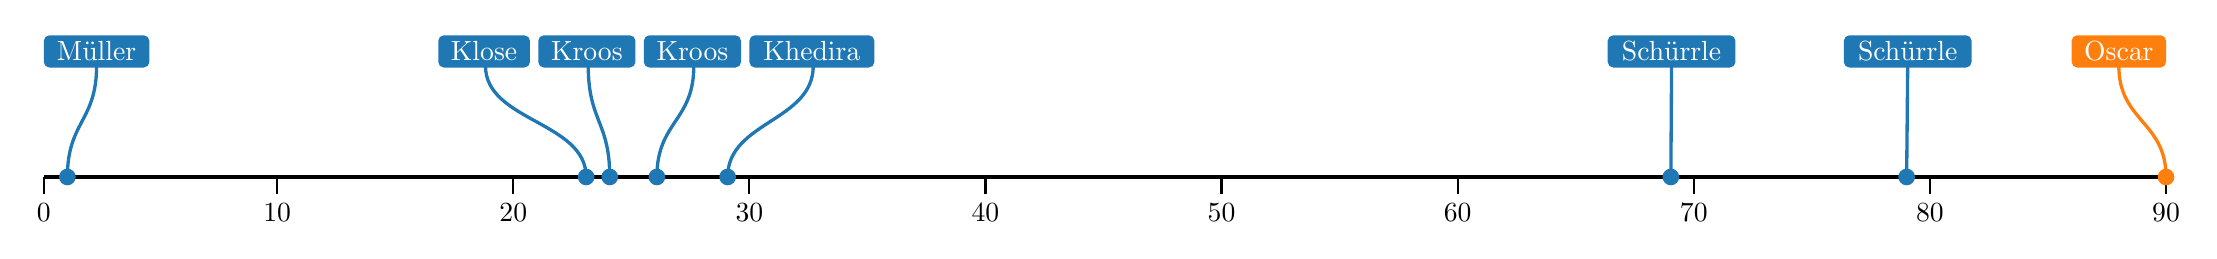
\begin{tikzpicture}[x=1bp,y=-1bp]

% shift for the margin
\begin{scope}[shift={(20, 20)}]
% main layer
\begin{scope}[shift={(0, 70)}]
% axis
\begin{scope}
\draw[very thick] (0, 0) -- (764, 0);
\end{scope}

% axis layer
\begin{scope}
\begin{scope}[shift={(0, 0)}]
\draw[thick] (0, 0) -- (0, -6pt)
node[anchor=north] {0};
\end{scope}
\begin{scope}[shift={(84, 0)}]
\draw[thick] (0, 0) -- (0, -6pt)
node[anchor=north] {10};
\end{scope}
\begin{scope}[shift={(169, 0)}]
\draw[thick] (0, 0) -- (0, -6pt)
node[anchor=north] {20};
\end{scope}
\begin{scope}[shift={(254, 0)}]
\draw[thick] (0, 0) -- (0, -6pt)
node[anchor=north] {30};
\end{scope}
\begin{scope}[shift={(339, 0)}]
\draw[thick] (0, 0) -- (0, -6pt)
node[anchor=north] {40};
\end{scope}
\begin{scope}[shift={(424, 0)}]
\draw[thick] (0, 0) -- (0, -6pt)
node[anchor=north] {50};
\end{scope}
\begin{scope}[shift={(509, 0)}]
\draw[thick] (0, 0) -- (0, -6pt)
node[anchor=north] {60};
\end{scope}
\begin{scope}[shift={(594, 0)}]
\draw[thick] (0, 0) -- (0, -6pt)
node[anchor=north] {70};
\end{scope}
\begin{scope}[shift={(679, 0)}]
\draw[thick] (0, 0) -- (0, -6pt)
node[anchor=north] {80};
\end{scope}
\begin{scope}[shift={(764, 0)}]
\draw[thick] (0, 0) -- (0, -6pt)
node[anchor=north] {90};
\end{scope}
\end{scope}

% link layer
\begin{scope}
\draw[color=linkColorA, very thick] (8.48888889, 0.00000000) .. controls
(8.48888889, -20.00000000) and (19.00000000, -20.00000000) .. (19.00000000, -40.00000000);
\draw[color=linkColorB, very thick] (195.24444444, 0.00000000) .. controls
(195.24444444, -20.00000000) and (159.00000000, -20.00000000) .. (159.00000000, -40.00000000);
\draw[color=linkColorC, very thick] (203.73333333, 0.00000000) .. controls
(203.73333333, -20.00000000) and (196.00000000, -20.00000000) .. (196.00000000, -40.00000000);
\draw[color=linkColorD, very thick] (220.71111111, 0.00000000) .. controls
(220.71111111, -20.00000000) and (234.00000000, -20.00000000) .. (234.00000000, -40.00000000);
\draw[color=linkColorE, very thick] (246.17777778, 0.00000000) .. controls
(246.17777778, -20.00000000) and (277.00000000, -20.00000000) .. (277.00000000, -40.00000000);
\draw[color=linkColorF, very thick] (585.73333333, 0.00000000) .. controls
(585.73333333, -20.00000000) and (586.00000000, -20.00000000) .. (586.00000000, -40.00000000);
\draw[color=linkColorG, very thick] (670.62222222, 0.00000000) .. controls
(670.62222222, -20.00000000) and (671.00000000, -20.00000000) .. (671.00000000, -40.00000000);
\draw[color=linkColorH, very thick] (764.00000000, 0.00000000) .. controls
(764.00000000, -20.00000000) and (747.00000000, -20.00000000) .. (747.00000000, -40.00000000);
\end{scope}

% label layer
\begin{scope}
\begin{scope}[shift={(0, -51)}]
\fill[color=labelBgColorA, rounded corners=2pt]
(0, 0) rectangle (38, 11.60416) node[midway, yshift=-.75bp, anchor=center, text=labelTextColorA] {\strut \textA};
\end{scope}
\begin{scope}[shift={(142, -51)}]
\fill[color=labelBgColorB, rounded corners=2pt]
(0, 0) rectangle (33, 11.60416) node[midway, yshift=-.75bp, anchor=center, text=labelTextColorB] {\strut \textB};
\end{scope}
\begin{scope}[shift={(178, -51)}]
\fill[color=labelBgColorC, rounded corners=2pt]
(0, 0) rectangle (35, 11.60416) node[midway, yshift=-.75bp, anchor=center, text=labelTextColorC] {\strut \textC};
\end{scope}
\begin{scope}[shift={(216, -51)}]
\fill[color=labelBgColorD, rounded corners=2pt]
(0, 0) rectangle (35, 11.60416) node[midway, yshift=-.75bp, anchor=center, text=labelTextColorD] {\strut \textD};
\end{scope}
\begin{scope}[shift={(254, -51)}]
\fill[color=labelBgColorE, rounded corners=2pt]
(0, 0) rectangle (45, 11.60416) node[midway, yshift=-.75bp, anchor=center, text=labelTextColorE] {\strut \textE};
\end{scope}
\begin{scope}[shift={(563, -51)}]
\fill[color=labelBgColorF, rounded corners=2pt]
(0, 0) rectangle (46, 11.60416) node[midway, yshift=-.75bp, anchor=center, text=labelTextColorF] {\strut \textF};
\end{scope}
\begin{scope}[shift={(648, -51)}]
\fill[color=labelBgColorG, rounded corners=2pt]
(0, 0) rectangle (46, 11.60416) node[midway, yshift=-.75bp, anchor=center, text=labelTextColorG] {\strut \textG};
\end{scope}
\begin{scope}[shift={(730, -51)}]
\fill[color=labelBgColorH, rounded corners=2pt]
(0, 0) rectangle (34, 11.60416) node[midway, yshift=-.75bp, anchor=center, text=labelTextColorH] {\strut \textH};
\end{scope}
\end{scope}

% dots
\begin{scope}
\draw node [circle, inner sep=0pt, minimum size=6bp, 
fill=dotColorA] at (8.488889, 0) {};
\draw node [circle, inner sep=0pt, minimum size=6bp, 
fill=dotColorB] at (195.244444, 0) {};
\draw node [circle, inner sep=0pt, minimum size=6bp, 
fill=dotColorC] at (203.733333, 0) {};
\draw node [circle, inner sep=0pt, minimum size=6bp, 
fill=dotColorD] at (220.711111, 0) {};
\draw node [circle, inner sep=0pt, minimum size=6bp, 
fill=dotColorE] at (246.177778, 0) {};
\draw node [circle, inner sep=0pt, minimum size=6bp, 
fill=dotColorF] at (585.733333, 0) {};
\draw node [circle, inner sep=0pt, minimum size=6bp, 
fill=dotColorG] at (670.622222, 0) {};
\draw node [circle, inner sep=0pt, minimum size=6bp, 
fill=dotColorH] at (764.000000, 0) {};
\end{scope}

\end{scope}
\end{scope}
\end{tikzpicture}
\end{document}